\documentclass{ieeeaccess}
\usepackage{cite}
\usepackage{amsmath,amssymb,amsfonts}
\usepackage{algorithmic}
\usepackage{graphicx}
\usepackage{textcomp}
\def\BibTeX{{\rm B\kern-.05em{\sc i\kern-.025em b}\kern-.08em
		T\kern-.1667em\lower.7ex\hbox{E}\kern-.125emX}}

\usepackage{lineno,hyperref}
\usepackage{subfig}
\usepackage{graphicx}
\usepackage{rotating}
\usepackage{multirow}
\usepackage{enumerate}
\usepackage{longtable}
\usepackage{comment}
\graphicspath{{./images/}}

\begin{document}

\begin{IEEEbiography}[{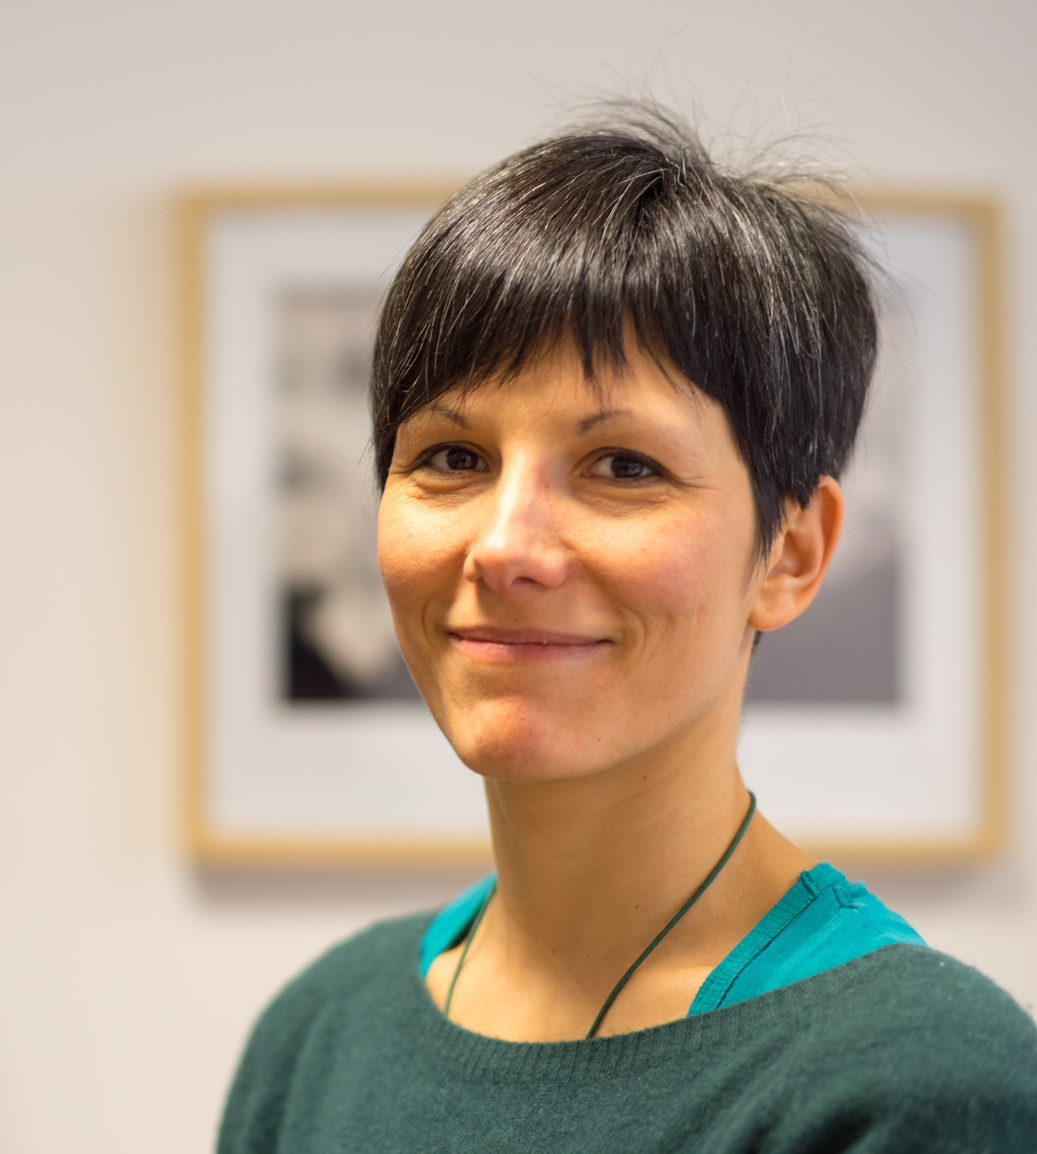
\includegraphics[width=1in,height=1.25in,clip,keepaspectratio]{Picture1.png}}]{Giulia Boato} is Associate Professor at the Department of Information Engineering and Computer Science (DISI) of the University of Trento (Italy). She is associate editor for the IEEE Transactions on Image Processing, for the ELSEVIER Signal Processing: Image Communication, and for the Journal of Electronic Imaging. Her research interests are focused on image and signal processing, with particular attention to multimedia data protection, data hiding and digital forensics, but also intelligent multidimensional data management and analysis. She is author of 120 papers in international conferences and journals, with H-index 22 (Google Scholar). She is elected member of the IEEE Multimedia Signal Processing Technical Committee (MMSP TC), of the IEEE Information Forensics and Security Technical Committee (IFS TC) and of the EURASIP Special Area Teams Biometrics, Data Forensics, and Security.
\end{IEEEbiography}

\begin{IEEEbiography}[{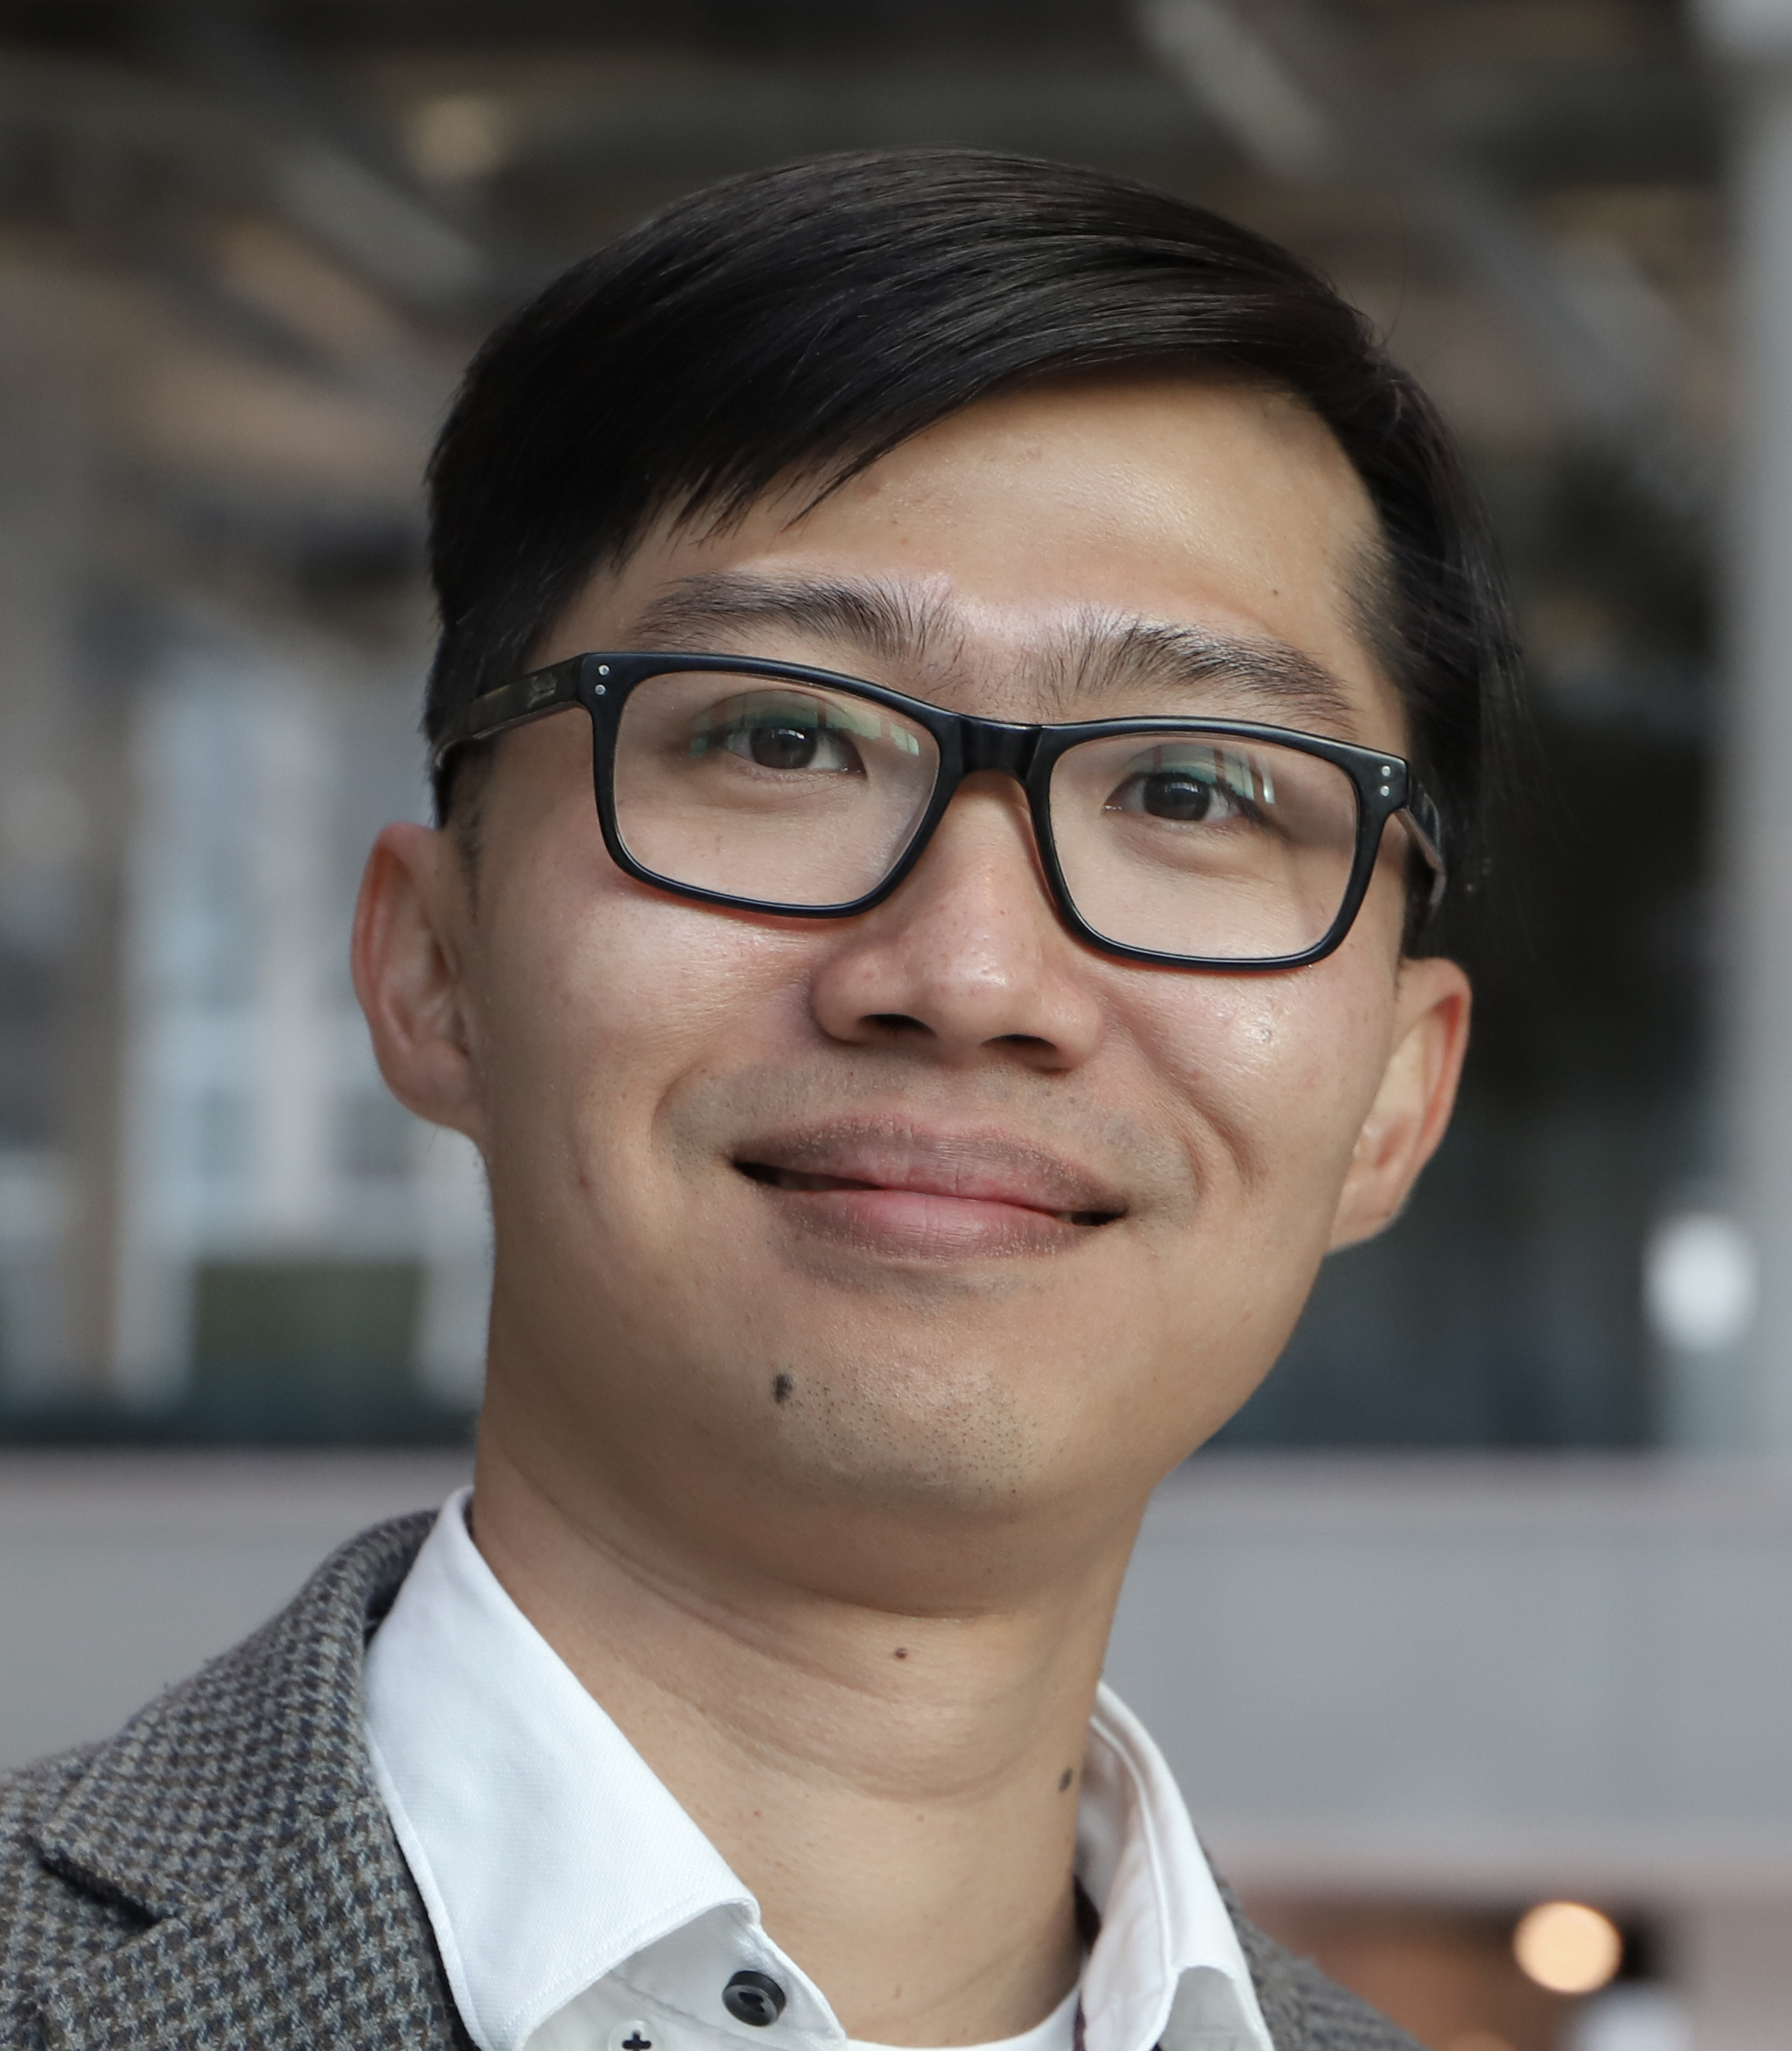
\includegraphics[width=1in,height=1.25in,clip,keepaspectratio]{Tien.jpg}}]{Duc-Tien Dang-Nguyen} is currently an Associate Professor at the Department of Information Science and Media Studies (Informedia), University of Bergen (Norway). His main area of expertise is on multimedia forensics, lifelogging, multimedia retrieval, and computer vision. 
%
He is author of 80 papers in international conferences and journals, with H-index~17 (Google Scholar, October 2019). He is member of IEEE Signal Processing, ACM, SIGIR, IAPR and INSTICC.  
He has organised and chaired over 20 workshops and special sessions, has been served as program committee for numerous international conferences and workshops, and has peer-reviewed for many top journals and conferences in the fields of lifelogging, multimedia forensics, and pattern recognition. Co-organiser of both the Multimedia Verification task, the NTCIR Lifelog task, the ImageClef Lifelog tasks, and many other MediaEval tasks. 
\end{IEEEbiography}


\begin{IEEEbiography}[{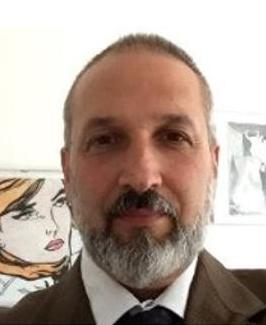
\includegraphics[width=1in,height=1.25in,clip,keepaspectratio]{denatale.jpg}}]{Francesco G.B. De Natale} was the Head of the Department of Information Engineering and Computer Science (DISI), University of Trento (Italy) from 2007 to 2010, where he currently leads the MMLab Research Laboratory. He is also a Professor of telecommunications with the University of Trento. His research interests include multimedia communications, where he published over 200 works in the major international journals and conferences. He is also a member of the Board of Governors of the CNIT Consortium. He has been an Associate Editor of the IEEE Transactions on Multimedia and the IEEE Transactions on Circuits and System for Video Technologies.
\end{IEEEbiography}

\end{document}